\section{Experimental Evaluation}\label{sec:exp}
We first apply our approaches to several real-world dataset and compare our method with uniform random sampling. Then we conduct several user studies on specific analysis tasks. 
\subsection{Case Study}
In this section, we evaluate our method by presenting the applications on two taxi trajectory datasets: Porto and Shenzhen. We compare the visualizations generated by the full dataset, random sampling and the proposed method from multiple levels of details. 
\subsubsection{Case of Porto Distinct}
Our first example uses taxi trajectories collected from 442 active taxis in Porto distinct, Portugal~\footnote{\url{http://www.geolink.pt/ecmlpkdd2015-challenge/dataset.html}}. The trajectories cover several cities in and around the Porto distinct and has been cleaned for further analysis.


\stitle{Overview of the Porto Distinct}
Figure~\ref{fig:teaser}(A) presents the visualization generated by the whole dataset, from which we can get an overview of the movement patterns in Porto district. For example, large number of trajectories are concentrated in the center of the figure(shown around Figure~\ref{fig:teaser}(A$_1$)), indicating that the most taxi activities are around the \UC{Porto City}. In addition, 
many trajectory clusters distributed across the land, which indicates the locations of other cities in Porto district(shown as the dashed circle in Figure~\ref{fig:teaser}(A)). 

We compare the $\avats$ with \textit{uniform random sampling} at the overview. 
Figure~\ref{fig:teaser}(C,E) show the visualization generated by uniform random sampling and $\avats$ respectively. Both of these two sampling methods take 0.01 as the sampling rate. The uniform random sampling almost only preserves the visual structure around the Porto City and the trajectories at the marginal regions are lost.
The visualization generated by $\avats$ looks close to the whole dataset. Not only the \UC{Porto City} but also the marginal city structures are well preserved, which are shown as the dash circles in Figure~\ref{fig:teaser}(E).
 
Furthermore, the color encoding further enhances the visualization by revealing the \QM{representativeness} of the trajectories.
As shown by the rectangle region in Figure~\ref{fig:teaser}(E), there is no clear pattern that can be discovered due to the dense concentration of massive trajectories. While in the same region of Figure~\ref{fig:teaser}(F), some trajectories with high representative scores are highlighted by dark orange color such as F$_1$, which indicates Avenida da Boavista, a main avenue in Porto City. 
%From the overview, $\avats$ can preserve the general structure very well in the comparison with uniform random sampling, and more information of the movement can be visualized with color encoding.
 
 
An important factor affecting the visual fidelity of sampling results is the sampling rate. Figure~\ref{fig:teaser}(C,B) show the sampling results of random method with sampling rate set as 0.01 and 0.001. With the decreasing of the sampling rate, the shape of the trajectory visualizations clearly shrink to the Porto City and result to the loss of visual fidelity at the marginal region. Figure~\ref{fig:teaser}(E,D) demonstrate the visualization of $\avats$ with the sampling rate of 0.01 and 0.001. We observe that when the sampling rate is decreased, the overview framework of the trajectories remains the same but the trajectories around Porto City are significantly removed since more \QM{blank space/gap} can be found around the Porto City as shown in the rectangle of Figure~\ref{fig:teaser}(D). 

\stitle{Detail view of Porto Distinct}
To demonstrate the effectiveness of $\avats$ at detail view, we select three regions of interest(as shown in the Figure\ref{fig:porto}(A)), which have different trajectory density and generate the visualization by setting the map level of 14) 
   
Region R3 is far away from Porto City and contains two other cities: Paredes and Penafiel. Region R3 has very few trajectories as shown in Figure~\ref{fig:porto}(D$_1$).  Compare with the visualization of full dataset, the random sampling almost misses all trajectories in this region(as shown in Figure~\ref{fig:porto}(D$_2$)). While $\vats$ samples much more trajectories than random sampling as shown in Figure~\ref{fig:porto}(D$_3$). However, some meaningful structure are still missing such as the trajectory bundle shown in Figure~\ref{fig:porto}(h), which is laid in on the road \QM{road name} connecting the two cities of Paredes and Penafiel. Further more, the trajectory structure of city Penafiel is not precisely preserved(shown as region g in Figure~\ref{fig:porto}(h)) because some  trajectory branches are missed.  
By setting the interpretation tolerance parameter as 64, $\avats$ generate a more confidential visualization than $\vats$ shown as Figure~\ref{fig:porto}(D$_4$). 

Region R2 is near to the center of Porto have are more taxi trajectories. There are three cities located in the region R2 including Ermesinde, Rio Tinto and Valongo.  
Figure~\ref{fig:porto}(C$_2$,C$_3$) present the visualization generated by $\avats$ with the interpretation tolerance parameters of 4 and 64. We observe that the visualization shown in Figure~\ref{fig:porto}(C$_3$) have more details trajectory branches than Figure~\ref{fig:porto}(C$_3$)(as shown in regions c,d of Figure~\ref{fig:porto}(C$_2$,C$_3$)). In this case, a larger interpretation tolerance parameter is more beneficial in preserving the details at this level. Furthermore, Figure~\ref{fig:porto}(C$_4$) shows the visualization of $\avats$($delta = 64$) with color encoding. In the comparison with Figure~\ref{fig:porto}(C$_3$), the visualization in Figure~\ref{fig:porto} further highlights the movement distribution. 
For instance, we observe that region $f$ in Figure~\ref{fig:porto}(C$_4$) has more deep colored trajectories than region $e$ and $g$, thus we inspect that city of Rio Tinto has more taxi trajectories than other two cities.
%For instance, we inspect that city Rio Tinto has more taxi trajectories than other two cities because.

The region R1 is the center of Porto city, which has the highest concentration of the trajectories and cause serious visual clutter if all trajectories are visualized(as shown in Figure\ref{fig:porto}(B$_1$)). $\avats$($delta = 4$) greatly alleviates the visual clutter and preserves the framework which basically follows the road network as shown in Figure~\ref{fig:porto}(B$_2$). Furthermore, when setting the interpretation tolerance parameter $delta$ as 64, the structure is more clear as shown in region b of Figure~\ref{fig:porto}(B$_3$,B$_4$), and have more trajectory details than $\avats$($delta = 4$) as shown in region $a$ of Figure~\ref{fig:porto}(B$_2$,B$_3$). The trajectories with color encoding further enhance the visualization thus the audiences can compare the traffic flow of two route more easily.   
 
 

\begin{figure*}[t]
	\centering
	\vspace{2mm}
	\includegraphics[width=0.98\textwidth]{pictures/experiment_study/case_porto.pdf}
	\caption{Visualization at dense and sparse region respectively.}
	\vspace{0mm}
	\label{fig:porto}
\end{figure*}

\begin{figure}[t]
	\centering
	\vspace{2mm}
	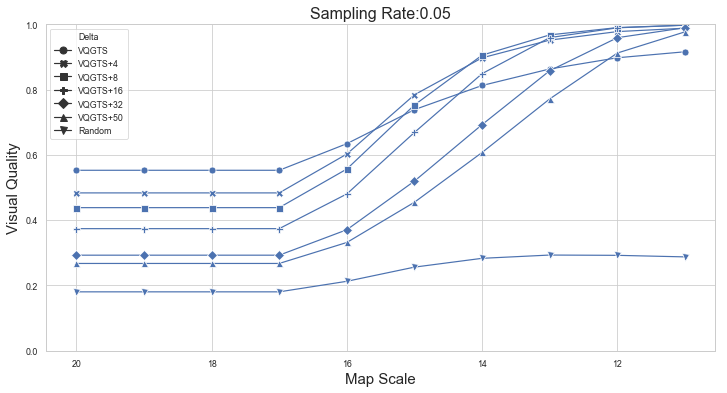
\includegraphics[width=0.45\textwidth]{pictures/experiment_study/quanlity.png}
	\caption{Visual quality chart. X axis indicates map scale from detail view to overview; y axis indicate the visual quality. }
	\vspace{0mm}
	\label{fig:quality_chart}
\end{figure}


\subsubsection{Shenzhen Trajectories}
We further evaluate the proposed approach using the taxi trajectories of Shenzhen, a booming city in the southern China and has very different urban form from Porto District. The dataset we used includes 428K taxi trajectories collected from \QM{**} taxis in one day. All the visualization generated by the sampling methods which sets the sampling rates as 0.01.
 
\stitle{Overview of Shenzhen}
Figure~\ref{fig:shenzhen}(A-D) present the overview visualization generated by whole dateset, random sampling, $\avats$ and $\avats$ with color encoding at the top level. The visualization of raw dataset(Figure~\ref{fig:shenzhen}(A)) shows the there are several dense trajectory clusters in southern districts of Shenzhen, including \textit{Baoan}, \textit{Nanshan}, \textit{Futian} and \textit{Luohu} districts, which are the most prosperous commercial zones of Shenzhen. Figure~\ref{fig:shenzhen}(B) presents the trajectories generated by random sampling. We observe that the most of the trajectories sampled by random sampling are located at the commercial zones. On the other hand, the trajectories at the north Shenzhen are missing, thus making the visualization visually different from the whole dataset.
$\avats$ outperforms random method by guaranteeing the spatial coverage of the whole trajectories thus result in a higher visual fidelity. Further more, some isolate trajectories are still preserved shown in Figure~\ref{fig:shenzhen}(C). $\avats$ with color is able to reveal the spatial distribution of the trajectories. For example, for the regions a, b in Figure~\ref{fig:shenzhen}(A or C), the visualization is unable to explain which region has more taxi activities because both of these two regions are fully covered by trajectories. In Figure~\ref{fig:shenzhen}(D), we find the more trajectories encoded by deep color are found in region a than that of region b, which indicates more trajectories can be found in region a than region b. 

\stitle{Detail view of Shenzhen}
Then we narrow down to the region of airport. Compare with visualization of whole dataset(shown as Figure~\ref{fig:shenzhen}(E)), the random sampling only preserves the trajectories pass through several routes with very high traffic flow(shown as Figure~\ref{fig:shenzhen}(F)).  Both $\avats$ and $\avats$ with color encoding can visualize the trajectory structure very well. The $\avats$ with color encoding further enriches the information by encoding the trajectory with color. For example, we can observe that there are more trajectories passing through G4 and G104 than Baoan Avenue, which is hard to be discovered from the Figure~\ref{fig:shenzhen}(E,F,G).  

Similarly, in the region near to the Shenzhen North Railway Station, the visualization generated by $\avats$ can reveal some road structure such as the \QM{round entrance to the motorway} shown as region c in Figure~\ref{fig:shenzhen}(K). With the color encoding, we can also easily discover that the road G94 have a higher road traffic flow than the Minzhi avenue and Mellon avenue as shown in Figure~\ref{fig:shenzhen}(L).

\begin{figure*}[t]
	\centering
	\vspace{2mm}
	\includegraphics[width=0.98\textwidth]{pictures/experiment_study/case_shenzhen.pdf}
	\caption{Case study of Shenzhen.}
	\vspace{0mm}
	\label{fig:shenzhen}
\end{figure*}

\subsection{User Study}\label{sec:user}
In this section, we conduct an extensive user study on three real-world applications, i.e., region center identification, reachable route inspection, and traffic flow detection, to demonstrate the superiority of our proposal.
We present our user study setting in Section~\ref{sec:uset}, and analyze the user study results in Section~\ref{sec:uret}.

%To further evaluate the effectiveness of $\avats$ from the the audience perspective, we conducted formal user studies to compare how users perform the urban exploration tasks with visualizations generated by whole dataset, random sampling and $\avats$.


\begin{figure}[t]
	\centering
	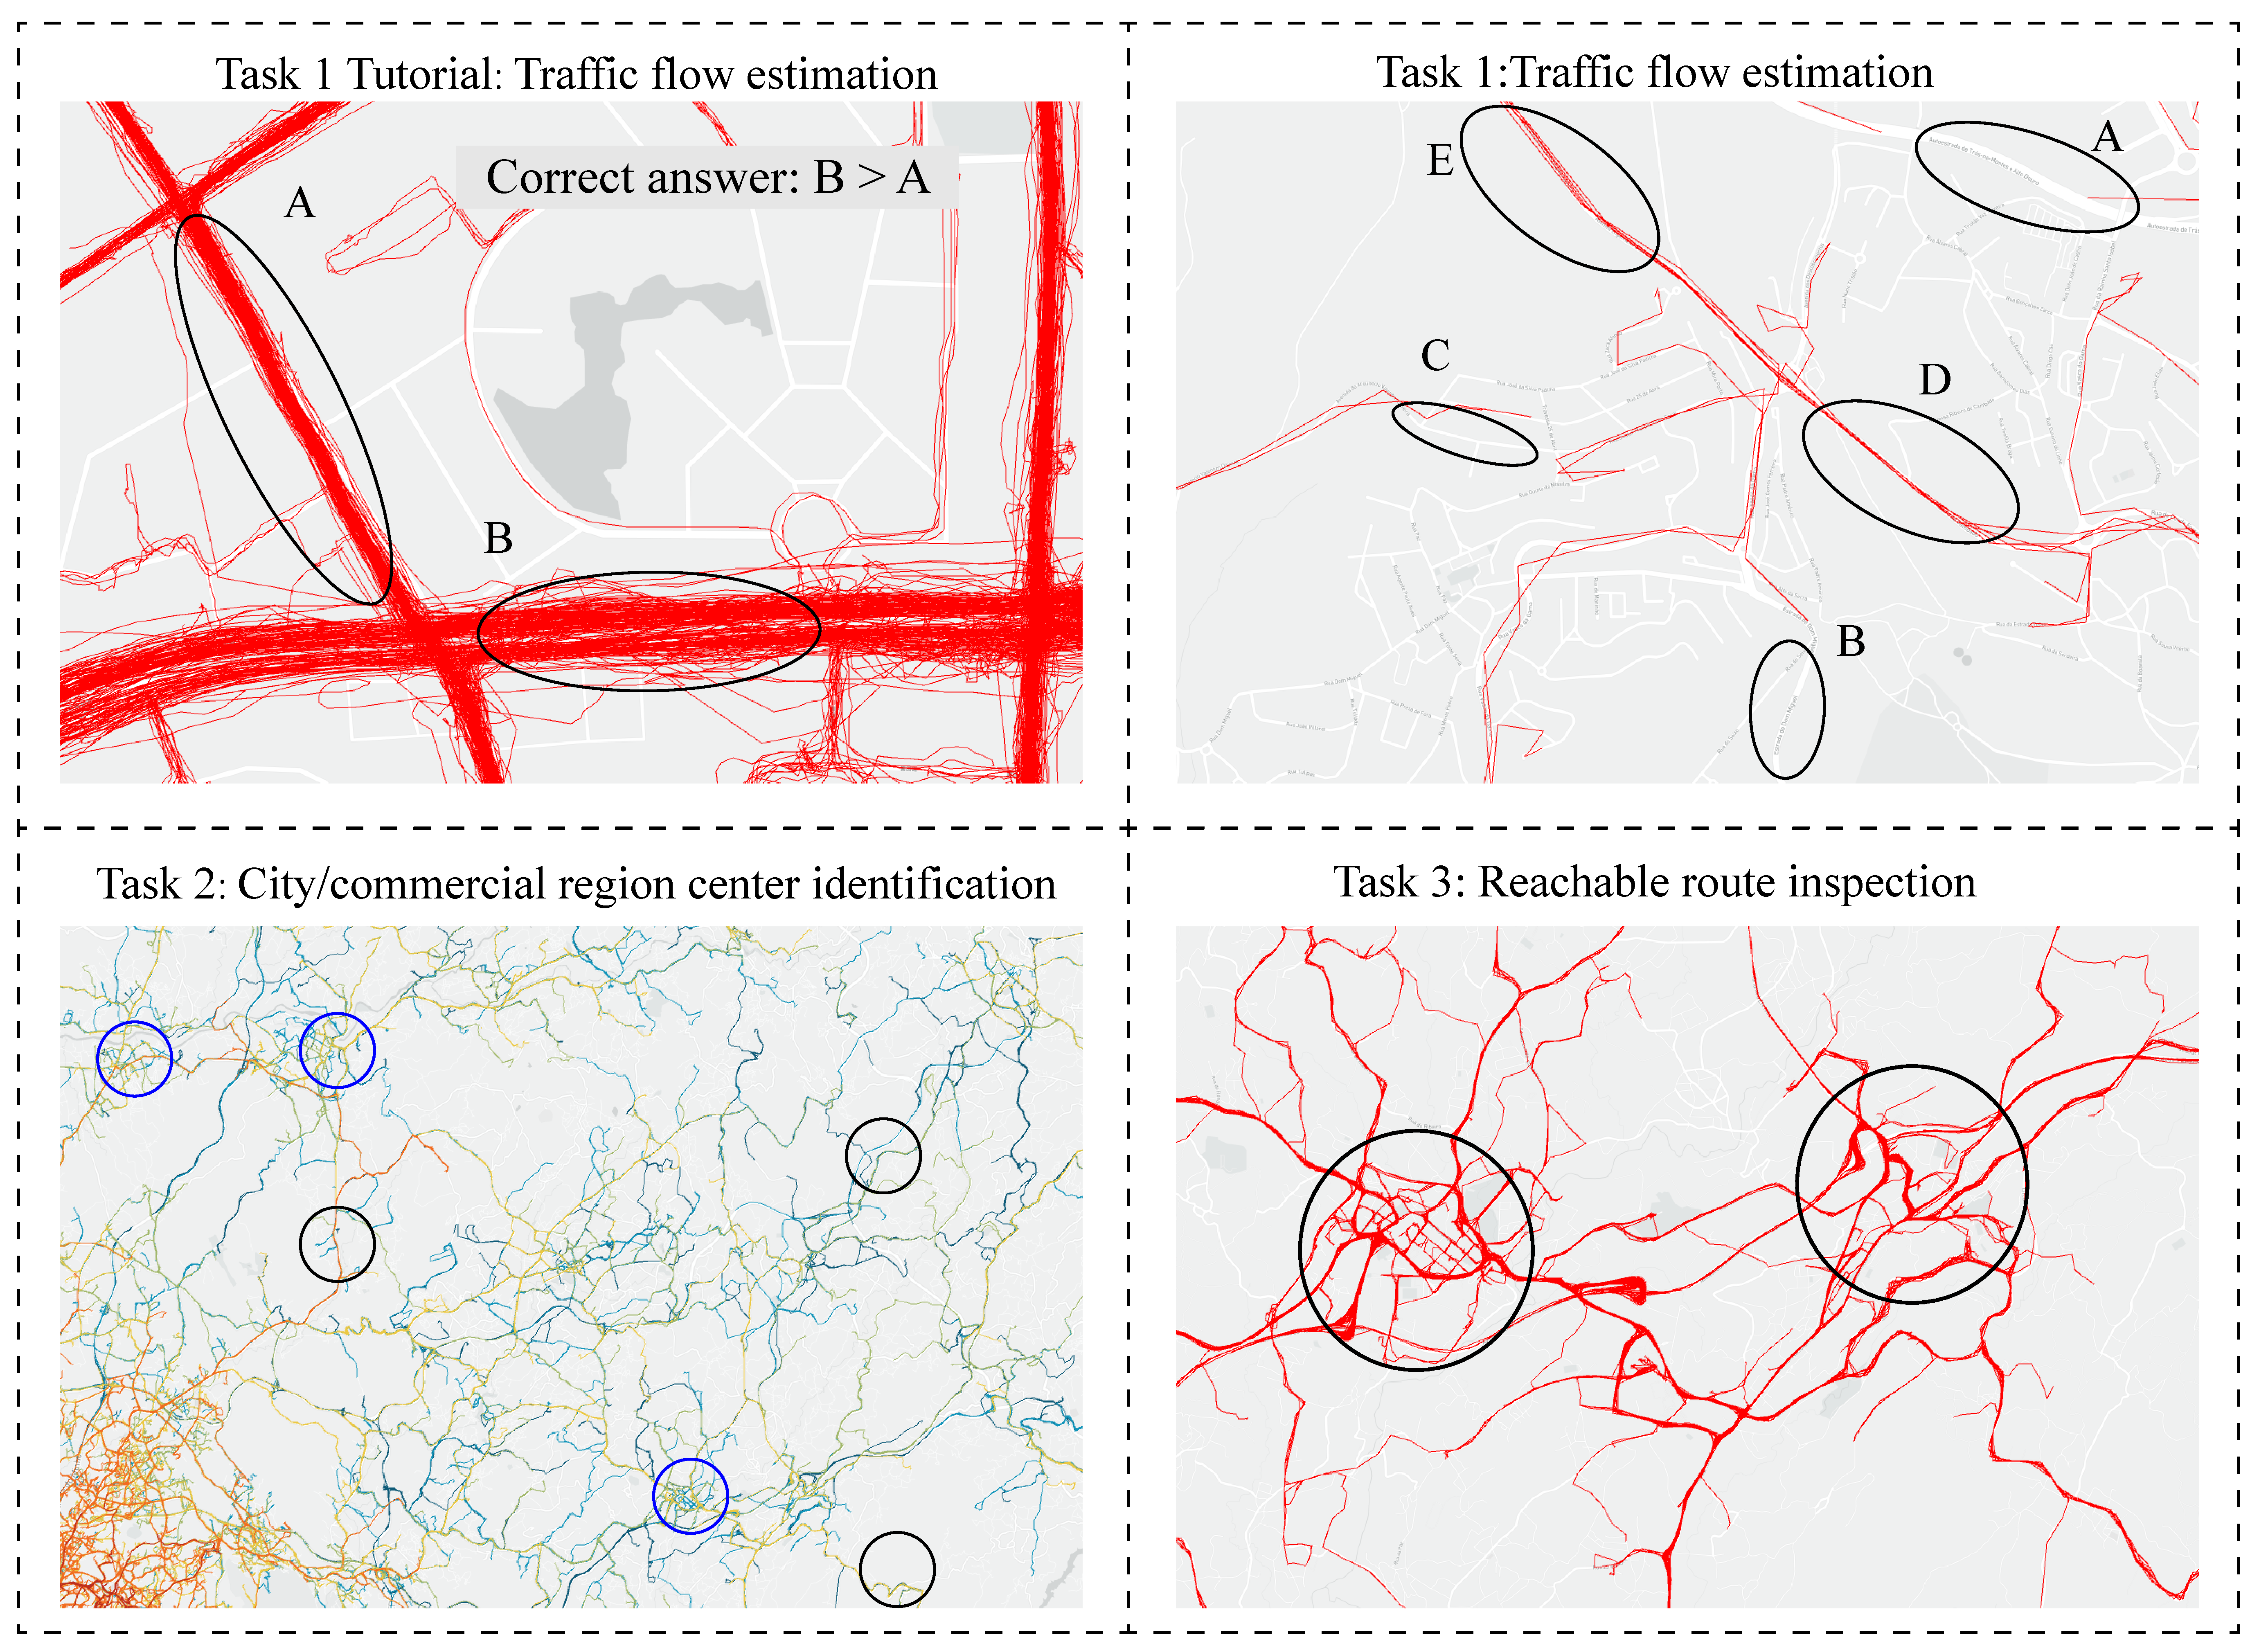
\includegraphics[width=0.48\textwidth]{pictures/user_study/interface.pdf}
	\caption{Three real-world applications in user study}
	\label{fig:apps}
\end{figure}

\subsubsection{User study setting}\label{sec:uset}

\stitle{Participants and apparatus}
We recruit 186 participants (24 females, 162 males, aged 18 to 29 with mean=21.16, standard derivation =1.48) with normal vision or normal corrected vision.
All participants have the background of computer science, 4.84\% of them have data visualization background.
The user study system is a web-based platform, which has the size-fixed interface and the participants perform the user study on their own  computers.
Considering the unfairness caused by different screen sizes, we recommend all participants to set the screen resolution as 1980*1080.
All images displayed on the interface have the same size 450*300.


\stitle{Studied visualization results}
We use the taxi trajectory dataset of \pt{} and \sz{} for the user study.
We study the visualization results which generated by different approaches in three real-world tasks.
We first introduce the studied data generation methods, then elaborate the tasks shortly.

The visualization results we investigated in user study are: (i) full dataset $\full$,
(ii) the result sets of $\rand$ (see Algorithm~\ref{alg:rand}),
(iii) the result sets of $\vats$ with performance optimizations (see Algorithm~\ref{alg:greedy}),
(iv) the result sets of $\avats$ without color encoding,
and (iv) the result sets of $\avats$ with color encoding (see Algorithm~\ref{alg:plus}), denotes as $\cavats$.
The sampling rate is $\alpha = 0.1\%$ and perception tolerance value $\delta = 64$ in all the visualization results in the user study section.
In each task, we use the identical regions with different visualized trajectories, which are returned from the above approaches.


\stitle{User study tasks}
All participants perform three tasks:  (T1) region center identification , (T2) reachable route inspection, and (T3) traffic flow estimation.
%as shown in Figure~\ref{fig:apps}(A), (B), and (C), respectively.

\sstitle{(T1) region center identification}
The center of the city or commercial region plays an important role in traffic management.
Consequently, the passing taxi trajectories of these centers are more than its surrounding regions, and results a star-shape cluster of trajectories in the visualization.
In this task, we randomly select 6 different regions which include city or commercial centers from \pt{} and \sz{}.
For each region, we ask the participate to identify the correct city/region center(s) in it.
As shown in Figure~\ref{fig:apps}(A), it asks the participate to identify 3 correct centers among these 6 cycles by clicking the corresponding cycles.
Specifically, T1 has 30 visualization views in total.
For each region of the visualization views,  we label the locations of the centers in it as the correct centers at first.
We then randomly select other areas which are not centers and far way from the correct centers, and label them as incorrect ones.
The number of correct centers in each visualization view is given to all participates.

%and remove these areas which too close to the correct ones,


% we have generated 145 visualizations(35 for T1, 75 for T2, 35 for T3) and 185 different questions(152 for T1, 21 for T2, 12 for T3).

\sstitle{(T2) reachable route inspection}
Intuitively, the visualized trajectories indicate the reachable routes of different regions.
In this task, we given a visualization view with two circular areas, as illustrated in Figure~\ref{fig:apps}(B),
then ask the participates to inspect the representative reachable routes between these two areas.
We assume the more trajectories in that route, the more representative it is.
For each visualization view, the number of reachable routes is given.
In T2, we randomly select 7 different regions which includes two or more cities/commercial districts.
In each region, we choose the identical two circular areas randomly for its 5 different visualization results.
%, which visualized the returned trajectory set of different approaches.


\sstitle{(T3) traffic flow comparison}
In practice, a road with large traffic flow has many passing trajectories, thus results to a denser and broader trajectory brunch in the visualization.
In the trajectory visualization with color encoding, such kind of pattern can also be highlighted by a concentration of trajectories with deep color.
It is important to preserve the traffic flow information during large trajectory visualization.
In this task, we ask the participates to compare the traffic flows in two roads by the given visualization results, as shown in Figure~\ref{fig:apps}(C).
In particular, the participants are asked to choose the road with large traffic flow by clicking the radio box.
They also can choose ``I am not sure'' if they cannot decided the answer.
T3 includes 5 randomly selected regions and each of them has clear road structure.
It has 25 visualization views and 60 road pair comparison in total.
We count the number of passing through trajectories in each road as the exact traffic flow in it.




%\textbf{T1. City/commercial region center identification.}
%% what participants do
%As shown by Figure~\ref{fig:user_study}(C), a visualization view was given and several regions were marked by circle. The participants needed to select the regions which could be city/commercial centers by click the corresponding circles. In each task, the number of correct regions were given.
%%Why possible
%The city or commercial region centers always have more passing trajectories from different directions than the surrounding regions, which results in the \UC{start-shape} cluster of trajectories in the visualization.
%%Generate the data
%To generate the test data of T1, we randomly chose several visualization views which contain city/commercial regions and labeled the locations of each city/commercial region center on the visualization as the correct locations first.  Then we randomly generated locations and remove the locations close to the correct locations, the remaining locations are the error locations. In each task of T1, with a given visualization, the same number of correct and wrong locations will be randomly selected.
%
%\textbf{T2. Reachable route inspection.}
%% what participants do
%Figure~\ref{fig:user_study}(D) shows the interface of T2, which includes a visualization and two circular regions. The users needed to draw several most representative reachable routes to connect the two regions. The number of the reachable routes is given.
%%Why possible
%The reachable routes indicate the routes connecting two regions, these routes must have the passing trajectories.
%%Generate the data
%To generate the test data, we randomly chose the visualization views which contain two or more city/commercial regions. In each task of T2, a visualization and two regions were randomly selected.

%\textbf{T3. Traffic flow estimation}.
%% what participants do
%As shown by Figure~\ref{fig:user_study}(B), with a given visualization, some road segments will be identified by ellipses(shown as~\ref{fig:user_study}(B)). Several road segment pairs were randomly selected and listed below the view. The participants were asked to choose the one with larger traffic flow by clicking the radio box. They can also choose ``I am not sure'' if they cannot decided the answer.
%%Why possible
%
%%Generate the data
%To generate the test data of T3,  we sampled and selected the visualization views which contain clear road structures. Then the number of trajectories passing through each road segment was counted as the traffic flow.



\stitle{User study procedure}
In the user study system, we first provide a brief introduction about the motivation, tasks and visual encoding scheme, then followed by three tasks.
In each task, we include a tutorial (with correct result) to help the participants familiarizing themselves with the interface, interaction and tasks.
For example, Figure~\ref{fig:apps}(D) shows a tutorial of T3 in Figure~\ref{fig:apps}(C), where the traffic flow in road A is smaller than it in road B, as the correct answer shown.
We then randomly choose different views with different questions in each task for different participates.
After she completed all the questions, her answers are collected and saved in the database for the result analysis.
At last, a post-interview were conducted to collect the feedback of the participants.
We refer the reviewers to our supplementary video for details of our user study procedure.

%The user study began with the introduction which introduces the motivation, tasks and visual encoding.
%Then the following sessions are divided into three blocks according to the task types. Each block starts with a task tutorial, in which the participants could perform several demo tasks, thus familiarizing themselves with the interface, interaction and tasks. For example, Figure~\ref{fig:user_study}(A) shows the demo task of T3, in which the users can check the correct answer after clicking the ``check'' button. After all the questions are finished, the answers and time usage are collected and saved in the database for the further analysis.

\subsubsection{User study result analysis}\label{sec:uret}
\TB{Figure~\ref{fig:accuracy} depicts the average accuracy of the different visualization approaches on different tasks from all user study participates.
Given a task with specified approach, we visualize the average accuracy of all questions by a colored circle and a line-segment to indicate the highest and lowest score of all questions of this task.}

\begin{figure}[t]
	\centering
	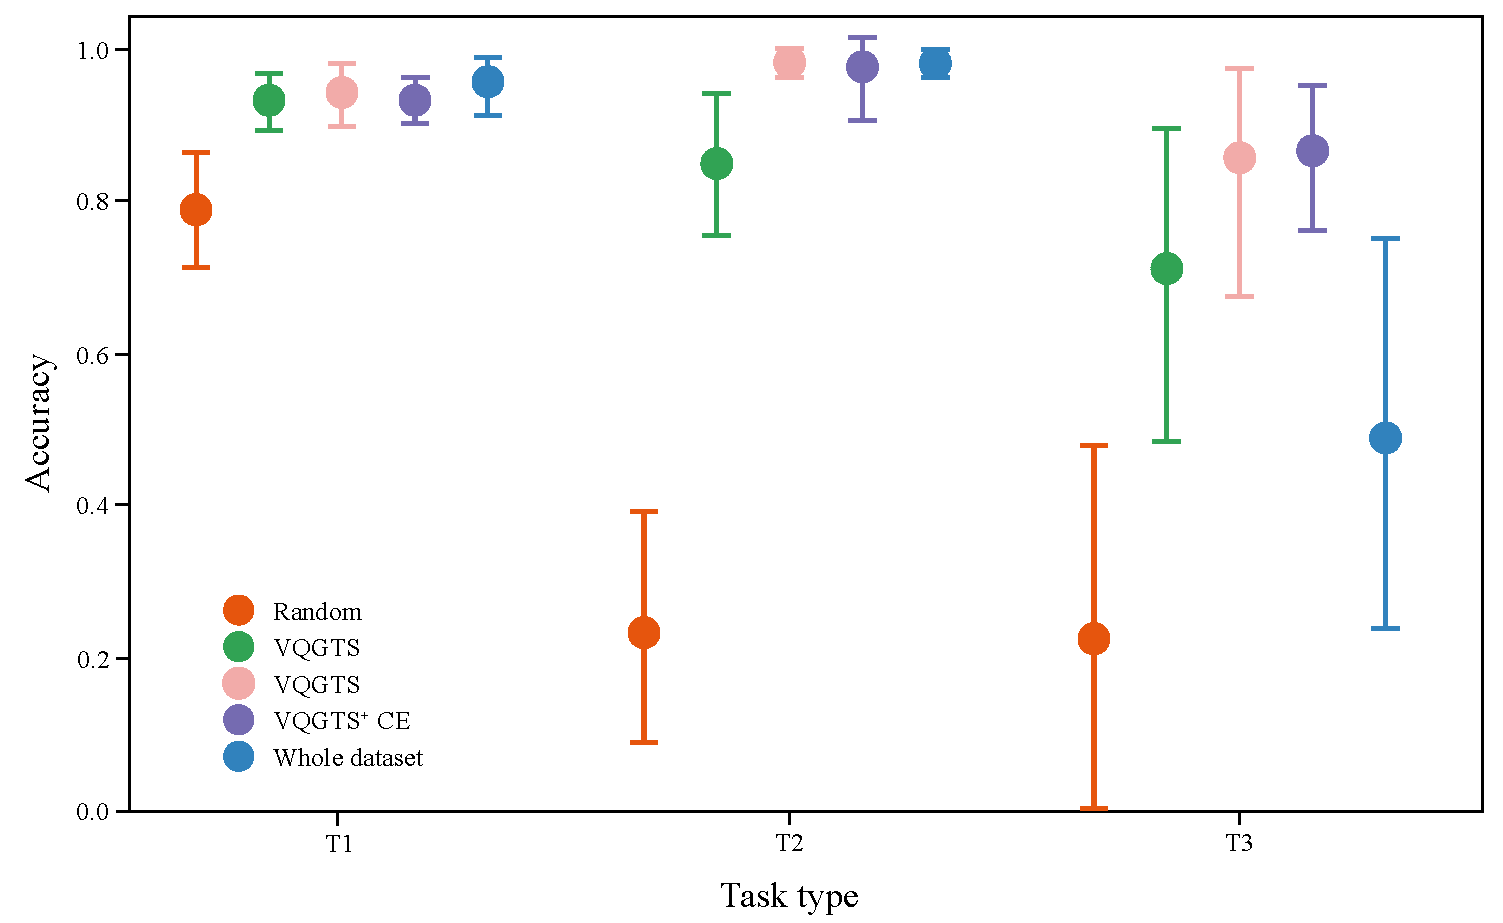
\includegraphics[width=0.44\textwidth]{pictures/user_study/accuracy.pdf}
	\caption{Average accuracy of three types of tasks. X axis indicates the task types. Y axis indicates the accuracy of different approaches.}
	\label{fig:accuracy}
\end{figure}



For T1 region center identification, the average accuracy of our proposed approaches (i.e., $\vats$, $\avats$, and $\cavats$) are higher than its of $\rand{}$ algorithm.
Moreover, our proposed approaches has a very close similar performance with visualizing the full dataset $\full$.
It means the visualized returning results of our proposed approaches worked as excellent as the full data visualization for the exploration of human activity center application.
We observed that the performance of $\cavats$ is slightly worse than performances of $\avats$ and $\full$.
In the post-interview, some of the participants say that the color of trajectories may distract user's attentions and make the cluster characteristics not obvious.


%the participants using all the three proposed methods had a very close performance with the participants using whole dataset, indicating the proposed methods can replace the whole dataset with a guaranteed performance in the exploration of human activity center with trajectory visualization.

For the reachable route inspection study in T2, it is no doubt the $\rand$ has the worst performance among these 5 visualization approaches as it lost many (if not all) detail information.
Unlike center identification in T1, the reachable route inspection in T2 are always performed at a fine-grained level of visualization,
which requires good preservation of the detail information, especially, for the sparse regions with few trajectories.
Thus, the advantages of our advanced approaches $\avats$ and $\cavats$ over $\vats$ become obvious and clear.
It owes to our advance approaches taken the data distribution and perception tolerance into consideration explicitly.
It also is worth to point out our $\avats$ (with average accuracy 0.968) outperforms the visualizations of $\full$ (with average accuracy 0.959) slightly.

%Interestingly,
%For the tasks of T2, $\avats$, $\avats$ with color encoding and the whole dataset all have similar accuracy scores which are far higher than random sampling.
%Moreover, $\avats$ and $\avats$ with color encoding also outperforms the $\vats$ clearly by taking the perception parameters into consideration.
% This results demonstrate the advantage of $\avats$ on the urban exploration at a detail level.


Visually, the task of traffic flow comparison in T3 are more difficult than T1 and T2.
It results in relative lower average accuracy for all approaches.  As expected, $\rand$ is the worst.
Interestingly, the average accuracy of visualization views of $\full$ is lower than our proposed approaches, i.e., $\vats,\avats$ and $\cavats$.
In the post-interview, the participants pointed out that many visualization views of $\full$ dataset had serious visual clutter,
which made it is impossible to compare the traffic flows in the two road segments.
The average accuracy of our proposed $\avats$ shows $\avats$ alleviated the visual clutter problem and preserved the clear structure.
$\cavats$ further highlighted the crowded road segments from the surroundings by color, which resulted it has the highest average accuracy in the task T3.

In summary, the qualitative user study of our proposal demonstrates the effectiveness of $\avats$ for large trajectory visualization by three real-world tasks.
All of our proposals ($\vats$, $\avats$, and $\cavats$) outperform the $\rand$ approach significantly.
In addition, the participates achieved equivalent or higher accuracy score in $\avats$ when comparing with the visualization of full dataset $\full$.


\subsection{Qualitative Evaluation}\label{sec:quality}
In this section, we conduct qualitative evaluation of our proposals on \pt{} and \sz{} trajectory datasets from two aspects: (i) the visual fidelity in different zoom levels,
and (ii) the running time with different sampling rates.

\begin{figure}
 \centering
 \small
 \begin{tabular}{cc}
   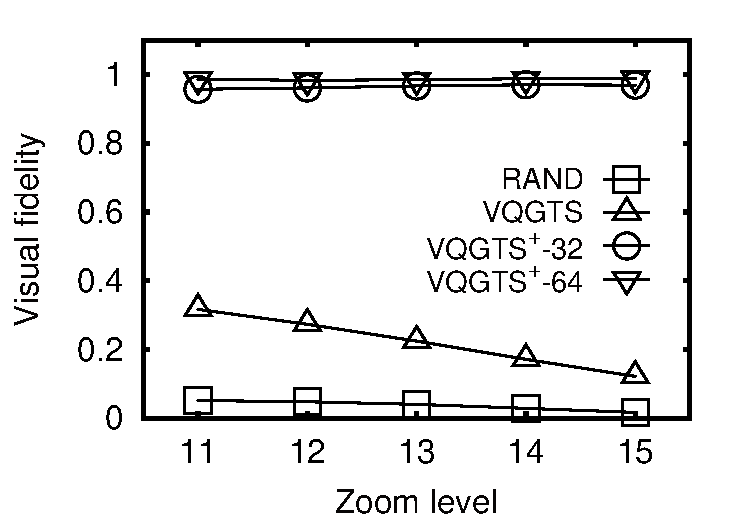
\includegraphics[width=0.48\columnwidth]{fporto}
   &
   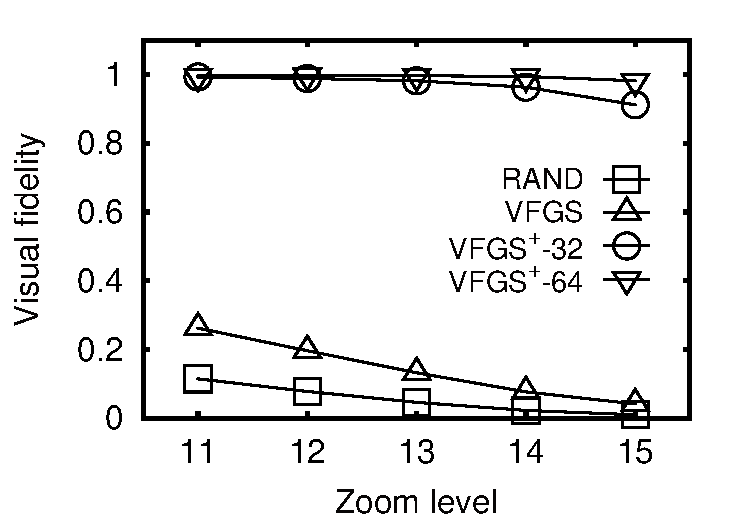
\includegraphics[width=0.48\columnwidth]{fshenzhen}
   \\
   (A) \pt{}
   &
   (B) \sz{}
 \end{tabular}
 \caption{Visual fidelity of proposed approaches}
 \label{fig:fidelity}
 \vspace{-4mm}
\end{figure}

\stitle{Visual fidelity evaluation}
We first evaluate the visual fidelity of our proposed methods.
We measure the visual fidelity of different approaches over the full dataset $\full$ by using the $loss()$ function we defined in Section~\ref{sec:def}.
Figure~\ref{fig:fidelity} (A) and (B) shows the visual fidelity of $\rand$, $\vats$, $\avats$ with $\delta=32$ and $\avats$ with $\delta=64$ from zoom level 11 to 15 in
\pt{} and \sz{}, respectively.
We can conclude that: (i) $\rand$ approach did not guarantee the visual fidelity of the result;
(ii) even $\vats$ offers theoretical visual fidelity guarantee w.r.t. the optimal sampled result set with given sampling rate, but it still has room for improving over the $\full$ dataset;
(iii) $\avats$ with $\delta=32$ and $\delta=64$ has excellent visual fidelity w.r.t. the $\full$ dataset. The minimum visual fidelity value is 0.95 and 0.91 in \pt{} and \sz{}, respectively.
It also confirms the superiority of our proposal;
and (iv) the visual fidelity of $\avats$ falls with the rising of zoom levels, e.g., from zoom level 11 to 15.
The reason is the higher zoom level, the more detail information are required.


\begin{figure}
 \centering
 \small
 \begin{tabular}{cc}
   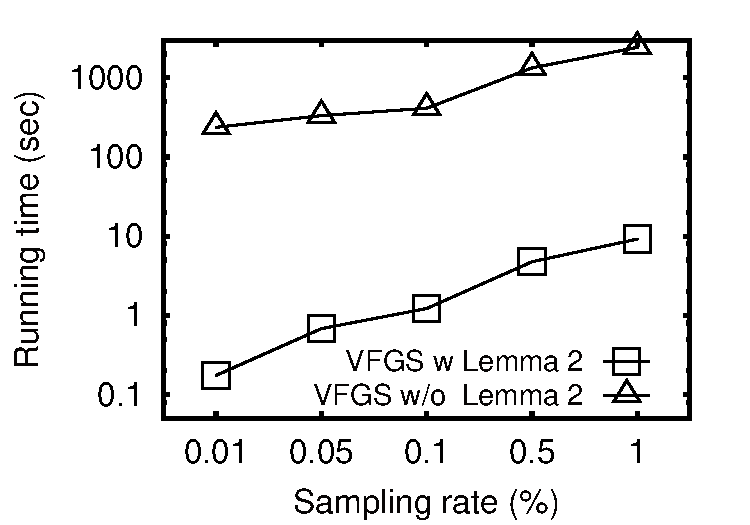
\includegraphics[width=0.48\columnwidth]{tporto}
   &
   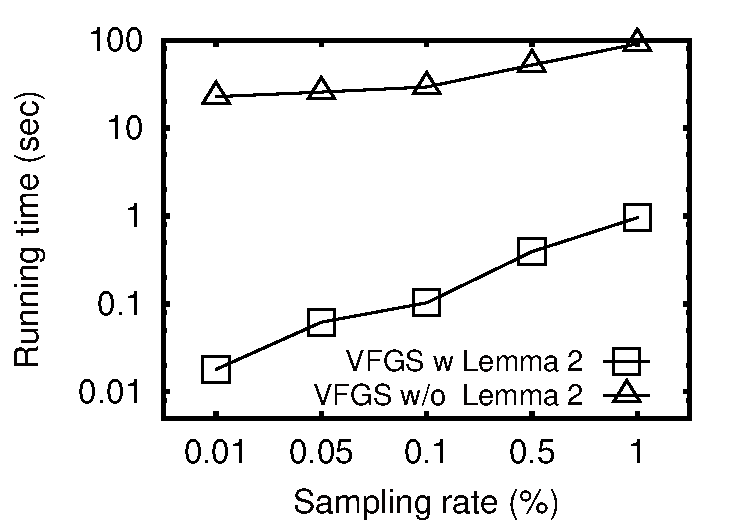
\includegraphics[width=0.48\columnwidth]{tshenzhen}
   \\
   (A) \pt{}
   &
   (B) \sz{}
 \end{tabular}
 \caption{The running time of $\vats$ with or without optimization techniques}
 \label{fig:cost}
 \vspace{-4mm}
\end{figure}


\stitle{Running time evaluation}
Last, we report the running time of our $\vats$ on two datasets: \pt{} and \sz{} by varying the sampling rate from $0.01\%$ to $1\%$.
It is no doubt our visual fidelity guaranteed sampling approach $\vats$ is quite slow without the performance optimizations in Section~\ref{sec:opt}.
Our optimized $\vats$ (e.g., $\vats$ with Lemma~\ref{lem:submodular}) outperform $\vats$ by one to three orders of magnitudes in both \pt{} and \sz{}, as shown in Figure~\ref{fig:cost}(A) and (B).
Finally, with excellent performance of our $\vats$, we conclude that our proposals provide interactive visualization for large trajectory data exploration, i.e., generate visualization results within seconds.


